\section{Chapter Overview}

An evaluation chapter connects the research questions to evidence. It should define the study design, variables, data sources, procedures, comparison conditions, and analysis methods before presenting results. This example uses invented data to demonstrate tables and a PGFPlots chart.

\section{Experimental Design}

Assume four methods are evaluated on three datasets. The independent variable is the selected method, and the primary dependent variable is performance measured as a percentage. Runtime is treated as a secondary outcome. A complete dissertation should also describe hardware, software versions, parameter settings, random seeds, inclusion criteria, and any data preprocessing required for reproduction.

\subsection{Evaluation Measures}

For observations \(x_1,\ldots,x_n\), the sample mean is

\begin{equation}
\label{eq:sample-mean}
\bar{x}=\frac{1}{n}\sum_{i=1}^{n}x_i.
\end{equation}

When results vary across repeated trials, report an appropriate measure of dispersion or uncertainty alongside the mean. The statistical method should match the research design and assumptions rather than being selected only after observing the results.

\section{Example Results}

Figure~\ref{fig:performance-plot} is generated directly in LaTeX with PGFPlots. This approach is useful for plots whose values are small enough to maintain in the source file. For large datasets or complex analyses, generate publication-quality PDF or PNG figures in the analysis software and store them in the relevant chapter's figure folder.

\begin{figure}[ht]
\centering
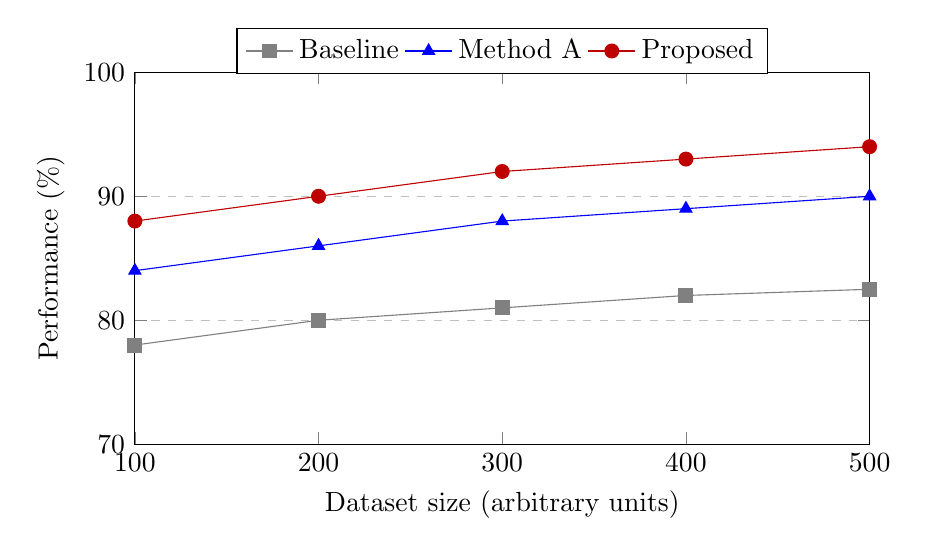
\begin{tikzpicture}
\begin{axis}[
    width=0.9\textwidth,
    height=0.52\textwidth,
    xlabel={Dataset size (arbitrary units)},
    ylabel={Performance (\%)},
    xmin=100, xmax=500,
    ymin=70, ymax=100,
    xtick={100,200,300,400,500},
    ymajorgrids=true,
    grid style=dashed,
    legend style={at={(0.5,1.12)},anchor=north,legend columns=3},
    mark size=2.5pt
]
\addplot[color=gray,mark=square*] coordinates {(100,78) (200,80) (300,81) (400,82) (500,82.5)};
\addlegendentry{Baseline}
\addplot[color=blue,mark=triangle*] coordinates {(100,84) (200,86) (300,88) (400,89) (500,90)};
\addlegendentry{Method A}
\addplot[color=red!75!black,mark=*] coordinates {(100,88) (200,90) (300,92) (400,93) (500,94)};
\addlegendentry{Proposed}
\end{axis}
\end{tikzpicture}
\caption{Illustrative performance trend produced with fictional data.}
\label{fig:performance-plot}
\end{figure}

Good figures make comparisons visible and avoid unnecessary decoration~\cite{tufte2001visual}. Captions should explain what is shown, while the body text should interpret the result. In this fictional example, all methods improve slightly as the horizontal variable increases, and the proposed method remains above the two comparison methods. No substantive claim should be made from these sample values.

\section{Threats to Validity and Limitations}

Limitations define the boundaries of an inference. Internal validity concerns whether the observed effect can be attributed to the proposed explanation. Construct validity concerns whether the selected measures represent the intended concept. External validity concerns whether findings transfer to other populations, settings, tasks, or time periods. Reliability and reproducibility concern whether procedures and results can be checked or repeated.

A limitations section should be specific. Instead of stating only that ``more research is needed,'' identify what is uncertain, why it is uncertain, how that uncertainty affects interpretation, and what evidence could reduce it.

\section{Reproducibility Checklist}

Before finalizing an empirical chapter, verify that it provides:

\begin{itemize}
    \item a clear connection between research questions and evaluation measures;
    \item enough information to understand the data and study procedure;
    \item justified comparison conditions and parameter choices;
    \item appropriate uncertainty, statistical analysis, or qualitative rigor;
    \item readable tables and figures with descriptive captions; and
    \item a candid account of limitations and scope.
\end{itemize}

\section{Institutional Support for Dissertation Development}
\label{sec:wcc-support}

The Writing and Communication Center (WCC) at Missouri University of
Science and Technology supports students and faculty working on projects
involving writing, speaking, and the presentation of ideas.\footnote{For
more information, visit the Missouri S\&T Writing and Communication Center:
\url{https://writingcenter.mst.edu/}}

\begin{figure}[ht]
    \centering
    
\includegraphics[width=\textwidth]{paper3/figs/WCC.png}
    \caption{Writing and Communication Center at Missouri University of
    Science and Technology.}
    \label{fig:wcc}
\end{figure}

Through individualized consultations and writing resources, the WCC helps
graduate students communicate their research clearly and effectively. This
LaTeX dissertation template and accompanying user guide were developed by
Keiwan Soltani, Ph.D. Candidate in Computer Science and Graduate Assistant
at the WCC, under the supervision of Dr. Jossalyn M. Gale, Director of the
Writing and Communication Center. The template extends the WCC's support
for graduate writers by providing a structured and reusable foundation for
organizing, formatting, and managing dissertations in LaTeX.

\section{Chapter Summary}

This chapter demonstrated an experimental structure, a labeled equation, a PGFPlots chart, result interpretation, and limitations. Chapter~\ref{ch:conclusion} closes the dissertation by synthesizing contributions and identifying future directions.
